%!TEX program = pdflatex
\documentclass{elegantpaper}

\usepackage{mathrsfs}




\title{Sky-camera based Cloud Movement Prediction and Sunlight Forecast}
\author{Yuchen Han(1824423)\\{\small Supervisor:Dr.Fei Cheng}}

\date{}




\begin{document}

\maketitle

\section{Summary of Proposal}

\subsection{Project Specification}
With the continuous reduction of power generation costs and the gradual maturity of technology, photovoltaic power has become one of the new green energy sources that meet the needs of human development. Photovoltaic power generation has strong randomness and discontinuity, which brings many unfavorable factors to photovoltaic grid connection.\cite{li2016multi} Therefore, it is necessary to predict the PV output power to reduce the impact of these unfavorable factors on the grid. Accurate prediction of photovoltaic power can provide important support for power grid scheduling, decision-making and effective reduction for the operating cost of power system.\cite{wan2015photovoltaic} It can improve the operating efficiency and economic benefits of the system.\\[2ex]
It is an important task for smart grids to forecast the short-term power output of a photovoltaic panel. Regular cameras which are mounted near solar panels can capture sky images to do short-term forecasting.\cite{yang2014solar} Estimating PV  based on the  relative position of sun and cloud, however, is quite challenging because of the changing weather patterns.\cite{huld2012new} Therefore, deep learning is used to learn the complicated relationship between sky images and the future photovoltaic power output. This project trains 3  neural networks( MLP, CNN, LSTM ) to do prediction. The input of neural networks is the sky pictures and corresponding photovoltaic power values. The project uses the input data and   trained neural networks to predict photovoltaic power in a very short term future. Python will be used to do data pre-processing,  images processing and result evaluation.\\[2ex]





\subsection{Specification Review}

From an environmental and economic point of view, renewable energy is very attractive. As an one of renewable energy, solar energy has great challenges to do prediction due to external factors such as changing weather.\cite{schweiger2017understanding} If  solar panel output power can be predicted precisely,  solar power can be fully developed so as to make great benefit for power grid management.\cite{wan2015photovoltaic} \\[2ex]
\\
	The problem of predicting solar panel output power has been widely studied in recent years. For  long-term forecasting, some researchers rely on the metadata which is supported by weather station or satellites.\cite{deo2017forecasting} 
	 However, the problem of predicting power output in short term, which is called short-term forecasting , is also important. It plays an important role  in managing the operation of smart grids, such as system integration. Short-term forecasting is able to ensuring power continuity and ramping electricity price management.\cite{antonanzas2016review} While some geosynchronous satellites do provide high temporal and spatial coverage, they are still an expensive option and may not be readily available.\\[2ex]
	 One way to solve this problem is to capture local weather conditions on solar panels with high spatial and temporal resolution, aligning the sky with a fixed camera and installing it near the panel.\cite{yang2014solar} However,  weather information cannot be provided by the facilities.  They simply provide images of the sky which will be analyzed to find out the relationship between these images and the photovoltaic power output. The cloud modeling can do help with this problem but it brings a great challenge to computer vision.\cite{fathi2015automated} \\[2ex]
	 In this work, we don't need to use traditional  techniques to explicitly model the movement of the cloud as the previous work. Instead,  algorithms are trained  automatically to learn the relationship between the the photovoltaic output  and sky's images and then predict future power output. The project uses multilayer perceptrons (MLPs), convolutional neural networks (CNNs), and long and short-term memory networks (LSTMs)  to solve the photovoltaic proximity prediction problems.\\[2ex]
	 




\subsection{Progress Report}

So far, datasets have already been obtained from solar panels. What's more, relevant literatures have been reviewed in order to determine the research topic and algorithms for this project.
 Considering one of the major tasks in this project is using  combination of neural networks to train data, some important algorithms (CNN, LSTM) have been reviewed and used into small samples, which makes contribute to build a well-performed algorithm architecture.\\[2ex]



\section{Data}
\subsection{Data source}
The data of this project is the sky images and corresponding photovoltaic power.
A photovoltaic panel was installed on the roof of EE building in Xi'an Jiaotong University. The sky camera was installed near the solar panel. 5 images can be captured every 5 seconds at different exposures({34,100,500,1000,2800}ms), which can obtain more detail information than single one. In the meantime, solar panel also records the corresponding photovoltaic values into a text file.This precess last for half years. 60 days' information is used in this project.\\[2ex]

The image content, image file names and photovoltaic values are shown as below.

\begin{figure}[!ht]
	\centering
	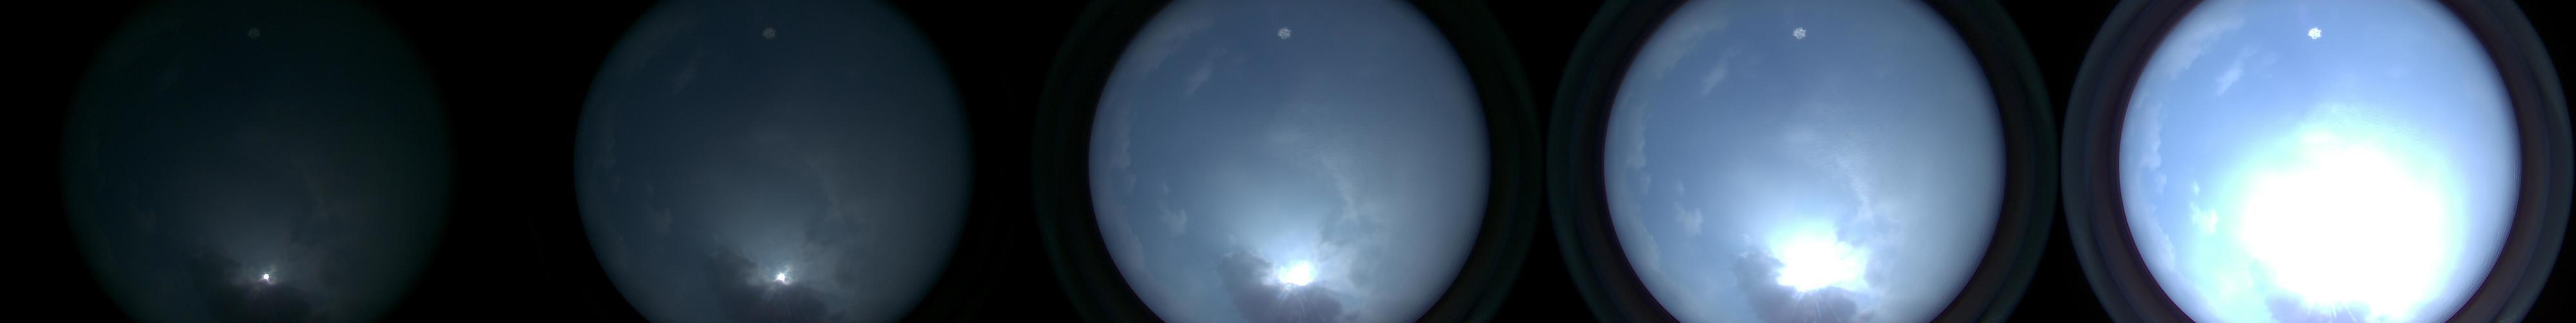
\includegraphics[width=\textwidth]{sun01.jpg}
	\caption{sky content\label{fig:sun}}
\end{figure}

\begin{figure}[!ht]
	\centering
	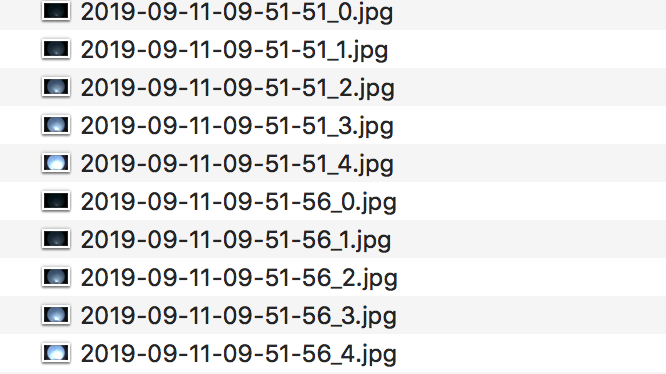
\includegraphics[width=0.6\textwidth]{sun_picture_01.png}
	\caption{sky images\label{fig:image file names}}
\end{figure}

\begin{figure}[!ht]
	\centering
	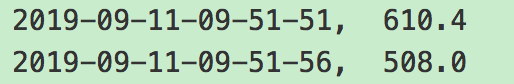
\includegraphics[width=0.6\textwidth]{irradiance_data.png}
	\caption{photovoltaic data\label{fig:photovoltaic}}
\end{figure}


 
\subsection{Data preprocessing}

The data was recorded every 5 seconds, but the project only uses data gathered every 1 minute. The images which contains sun and cloud should be taken into consideration. If weather is sunny, rainy or overcast, the photovoltaic is easy to obtain and keeps stable. Therefore, these images are dropped according to the corresponding photovoltaic value.\\[2ex]


\section{DESIGN OF THE PROPOSED ALGORITHM}


\subsection{MLP with past photovoltaic values}
MLP(multi-layer perceptron) are comprised several layers of neurons. Data is fed to the input layer, there may be more than one hidden layers providing levels of abstraction, and predictions are made on the output layer, also called the visible layer.\cite{yilmaz2009pitch} Here is the structure of MLP.

\begin{figure}[!ht]
	\centering
	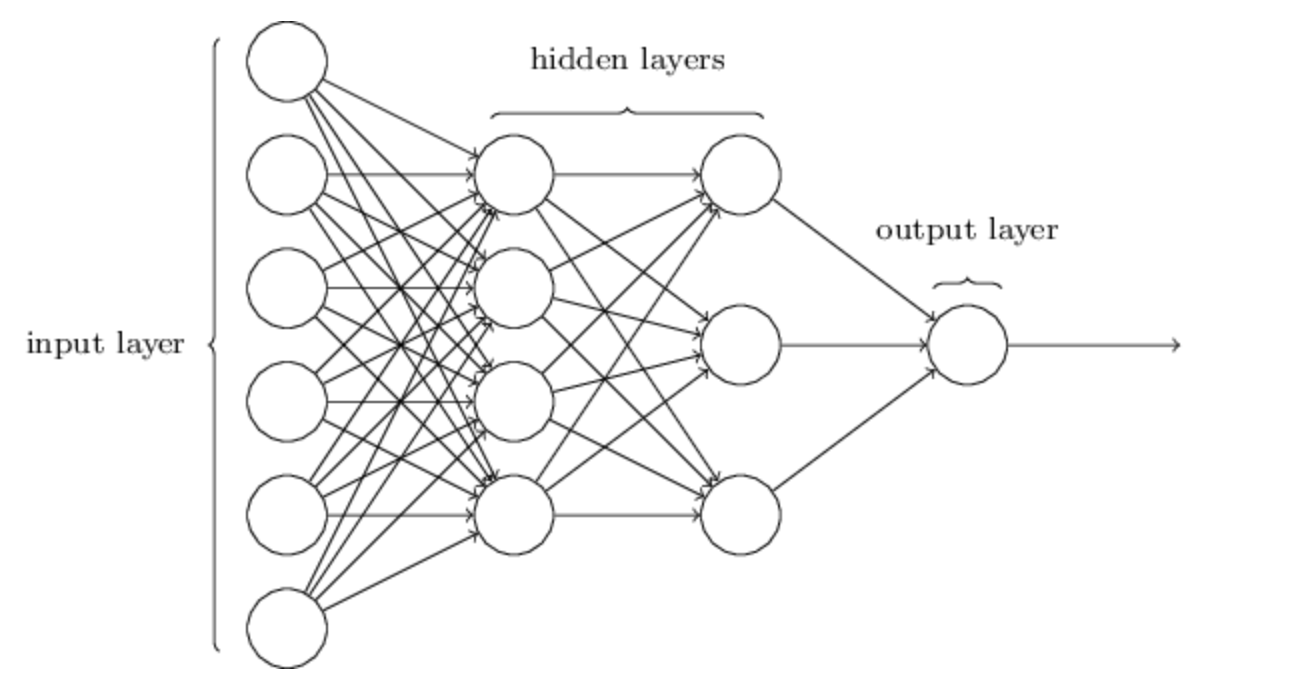
\includegraphics[width=0.6\textwidth]{mlp.png}
	\caption{basic MLP structure\label{fig:mlp}}
\end{figure}



The input of this model is historical photovoltaic power values, which is referred as $p$ to predict the variation $\bigtriangleup \hat{p_{t0}}$. This $m\times n \times 1$ MLP network contains two hidden layers $m$ and $n$, one output layer. The value $m = n = 32$ performs well in this network. After these two hidden layers, normalization, the “tanh” activation function are used.In the output layer, the network uses “sigmoid” activation function. L2 distance is applied to minimize values between the estimated values and the ground truth.\\[1.5ex]
$L_{\bigtriangleup p_{t0}}=\left \| \bigtriangleup \hat{p_{t0}}-\bigtriangleup p_{t0} \right \|  ^{2}$ \\


\subsection{CNN}

Although MLP network can use historical power value $p$ as input to do prediction, it has no relevance with images. The procedure will lose many feathers. Therefore, convolutional neural network(cnn) will be applied in order to solve this problems.  \\[2ex]


In machine learning area, the convolutional neural network is a deep artificial neural network , which can perform image processing with large data volume.\cite{quan2016fusionnet} The convolutional neural network is improved based on the BP neural network.\cite{howard2013some} Both networks use the forward propagation algorithm to calculate the output value and the backward propagation algorithm to adjust the weight and offset. The difference between convolutional neural networks and BP neural networks is the way in which neural units are connected. \cite{Ketkar2017Convolutional} The neural units between adjacent network layers in a convolutional neural network are locally connected, which is different from the way neural units are connected in a BP network. All neural units of the BP network are interconnected. In a convolutional neural network, the sensing area of the neural unit originates from a part of the neural unit of the previous network layer. The convolutional neural network structure contains several convolution layers, pooling layers, activation layer, fully connected layers.\cite{lin2013network} \\[2ex]

Therefore, CNN is an appropriate model to extract pictures' information. Then this project uses a combination of CNN with MLP to learn information through the images and  photovoltaic values. Here is the structure of CNN.\\[2ex]


\begin{figure}[!ht]
	\centering
	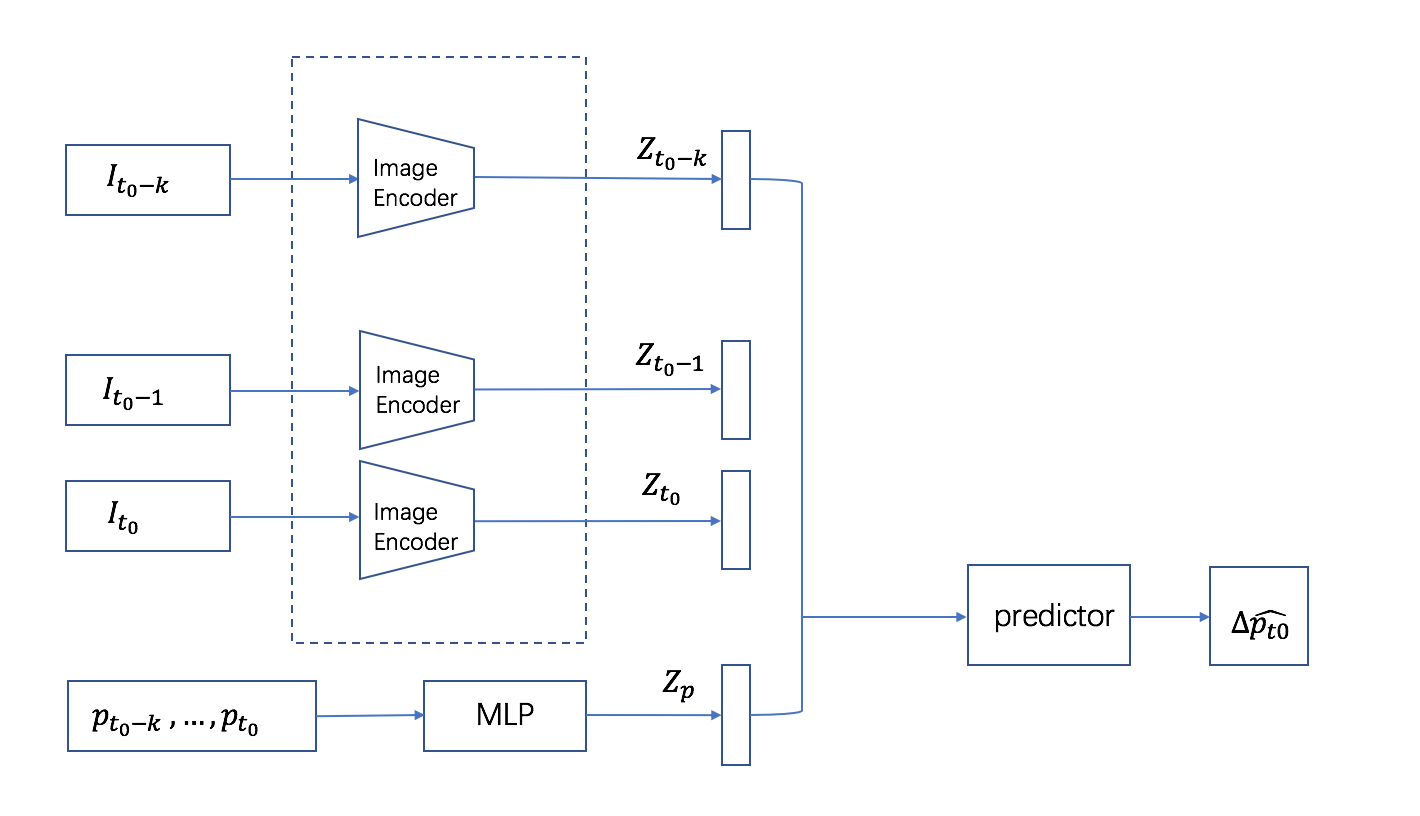
\includegraphics[width=1.0\textwidth]{cnn_mlp.png}
	\caption{CNN + MLP structure\label{fig:cnn_mlp}}
\end{figure}

The image encoder takes 2D image vector as input. After two convolutions, the image information is compressed into a vector $Z_{i}$. The first filter is $5\times5\times64$ and the second filter is $5\times5\times128$. There are 2 pooling layers, which uses $2\times2$ max pooling.\\
Here is the structure of Image encoder.

\begin{figure}[!ht]
	\centering
	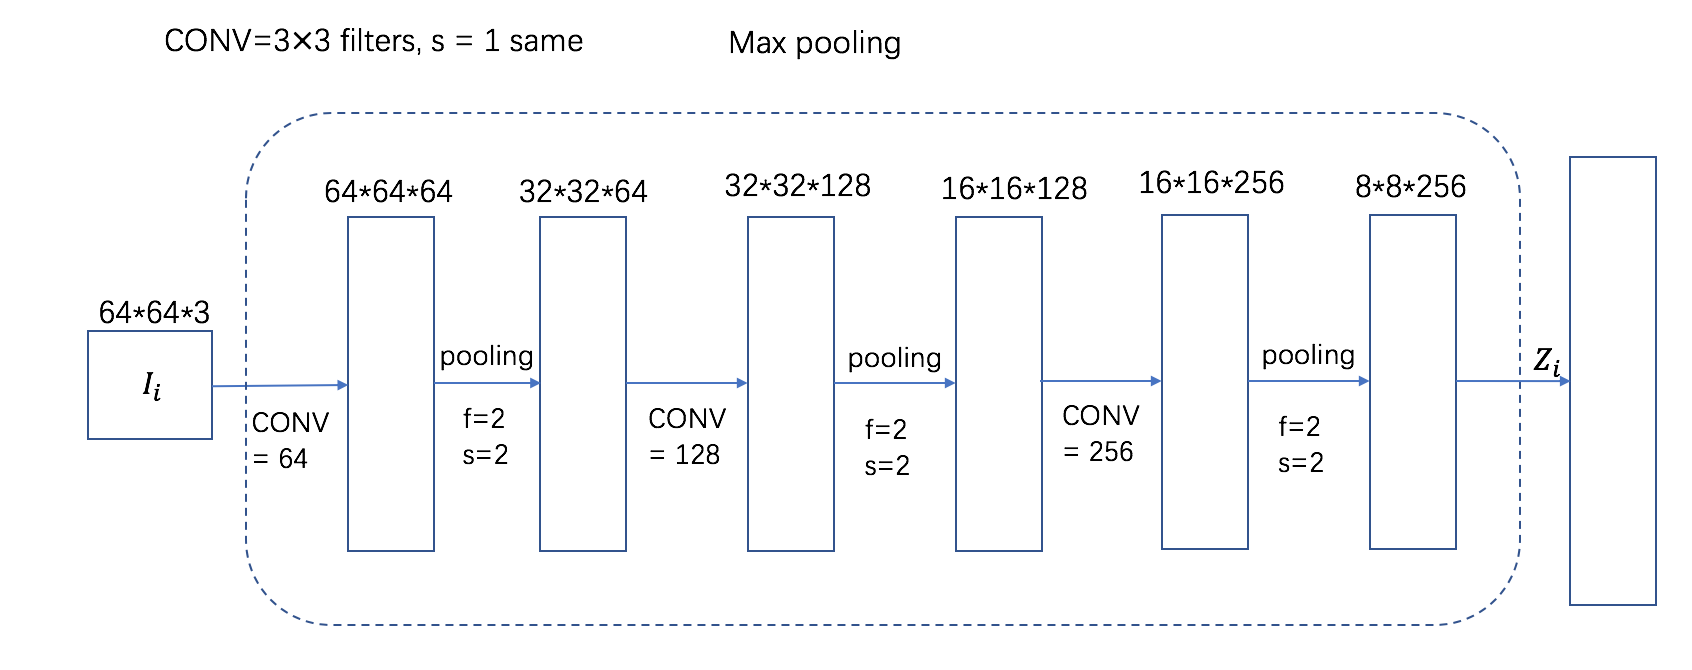
\includegraphics[width=1.0\textwidth]{predictor.png}
	\caption{Image encoder structure\label{fig:Image encoder}}
\end{figure}



The combination architecture contains 2 parts, MLP which has mentioned in last chapter and CNN part. For CNN part, images $I_{i}$ is taken as input, after which the input data is transformed into vector $Z_{i}$ through Image encoder. $i\in \left \{ t_{0}-k, ... , t_{0} \right \}$ Each image will use same set of weights. Power values will be transformed into $Z_{p}$ by MLP. $Z_{p}$ and $\left \{ z_{t_{0}-k}, ... , z_{t_{0}} \right \}$ are fed to the predictor. The predictor can be seen as the other MLP network. Its structure is $n \times n \times n \times 1$ with 3 layers. The combined model aims to learn the spatial and temporal changes so as to make precise prediction variation $\bigtriangleup \hat{p_{t0}}$.\\[2ex]


\subsection{LSTM}

The CNN models consider the image information and power values, however, temporal information does not take into consideration. In this part, temporal information will be used as another feather to feed the model.\\[2ex]

The LSTM (Long short term memory) is a special type of RNN.\cite{liu2018wind} It is suitable for processing and predicting the case where the interval and delay in the time series are relatively long.\cite{li2018prediction} The LSTM network adds input threshold, forgetting threshold and output threshold to the algorithm, so that the weight of its own loop is changed.\cite{gers1999learning} LSTM allows the network to forget the information that has been accumulated so as to avoid the problem of gradient disappearance or gradient expansion. Each hidden unit is replaced by a Cell with memory function. Each unit is placed with an input gate, an forgetting gate and an output gate.\cite{wang2018research} The three gates use the sigmoid activation function to control the transmission of information in the network and assign it to the current a certain amount of information at a time, and then allocated to the information needed by the network at the next moment.\cite{zhang2018use} \\[2ex]

For LSTM network,  $z_{t_{i}}$ are no longer the vectors used into feed the model. Instead, the 2-layer LSTM network is applied in the algorithm architecture. Here is the structure of LSTM.

\begin{figure}[!ht]
	\centering
	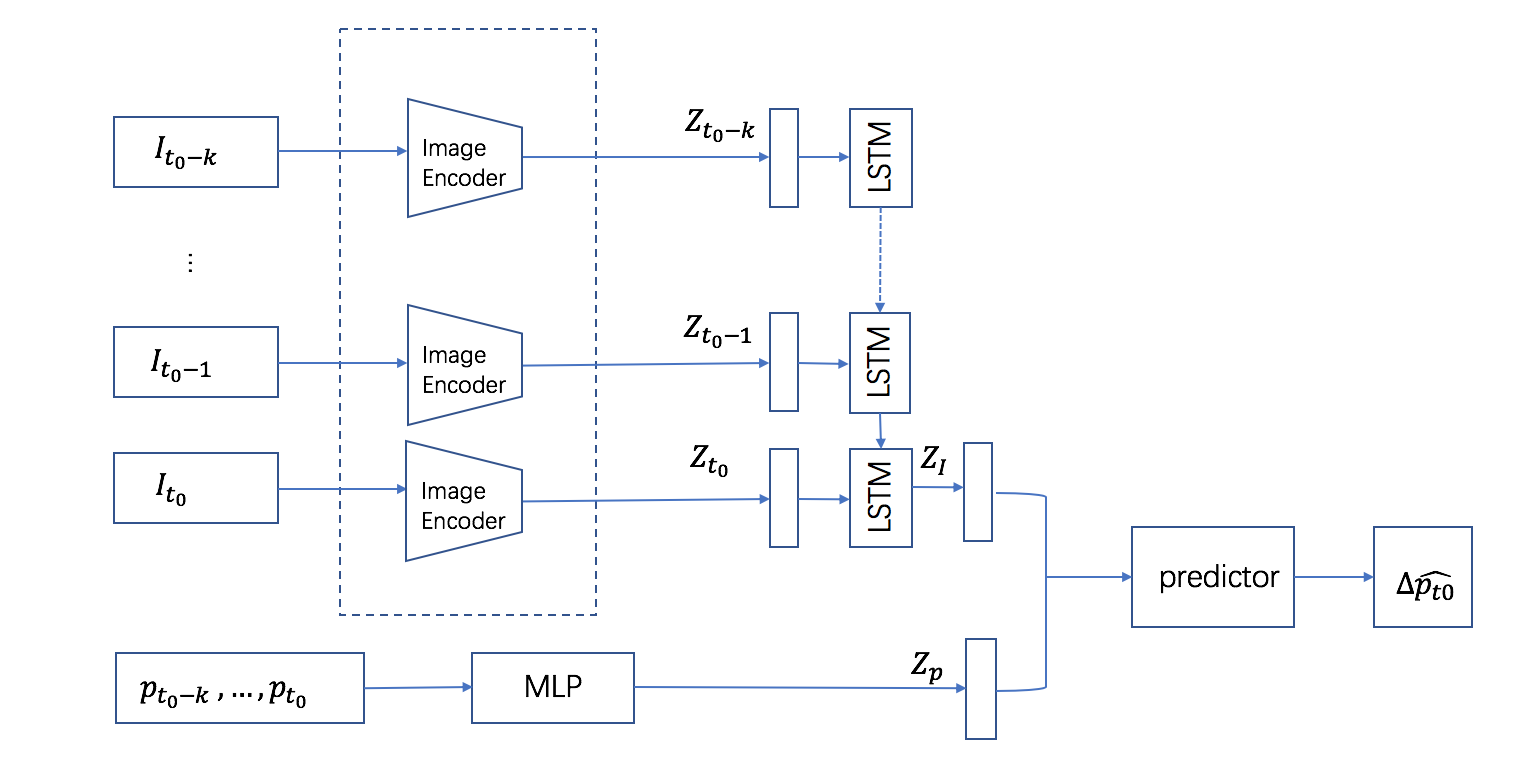
\includegraphics[width=1.0\textwidth]{lstm.png}
	\caption{LSTM structure\label{fig:lstm}}
\end{figure}

LSTM is good at getting the structure of sequences. After the data being processed, $z_{t_{I}}$ has all the past latent temporal information. Then $z_{t_{I}}$ and $z_{t_{p}}$ are concatenated to train the final network through a predictor to predict  $\bigtriangleup \hat{p_{t0}}$. The loss function remains the same as $L_{\bigtriangleup p_{t0}}=\left \| \bigtriangleup \hat{p_{t0}}-\bigtriangleup p_{t0} \right \|  ^{2}$ \\.



\section{Evaluation}
For  test data sets, there are three different weather condition categories: sunny, partially cloudy, and overcast. The "sunny" is defined as the days when the average cloud level is below $10\%$, "partially cloudy” is between $10\%$ and $90\%$ and “overcast” is completely cloudy. The following metrics are used to do evaluation.\\[2ex]
The “mean absolute error” (MAE) is the average of absolute errors, which can reflect the actual situation of the prediction value error well.\\[1.5ex]

$MAE=\frac{1}{N}\times\sum_{i=1}^{N}\left | p_{i}-\widehat{p_{i}} \right |$ \\[1.5ex]

The “root mean squared error” (RMSE) Is the square root of the deviation of the observed value from the true value and the ratio of the observed number m.It is used to measure the deviation between the observed value and the truth value. \\[1.5ex]

$RMSE=\sqrt{\frac{1}{N}\times\sum_{i=1}^{N} (p_{i}-\widehat{p_{i}})^{2}}$ \\[1.5ex]


RMSE is equivalent to the L2 norm, and MAE is equivalent to the L1 norm. The higher the number, the more the calculation results are related to the larger value, and the smaller the value is ignored. Therefore, RMSE is more sensitive to outliers than MAE. \\[1.5ex]

These two methods' performance will be estimated by The “forecast skill score” (SS).\\
$SS=\left ( 1-\frac{prediction}{baseline} \right )\times100\%$ \\[1.5ex]

The skill score (SS-MAE, SS-RMSE) will be used to compare the result of 3 algorithms.For the skill score, the baseline is stable. In the experiment period, each model was individually trained and the best performing validation) model  was selected from training procedure.




\section{Implementation detail}

The implementation of this project will be mainly in python. Keras will be used to implement MLP,CNN,Lstm as it is highly encapsulated and speed is very high. 
Several libraries such as matplotlib, sklearn and numpy will also be used to transform vectors and do visualization. For experiment, the data will run in the environment with 1080Ti GPU.


\section{Review of project plan}

 Since most of the algorithm work has been completed, subsequent efforts will be focused mainly on experiment and data analysis. The chart below shows the schedule for the whole work.\\

 The gantt chart in appendix A shows that most of the work has been completed and the future plan.
 
 

\bibliographystyle{ieeetr}
\bibliography{wp_ref}







 \appendix
 % \renewcommand{\appendixname}{Appendix~\Alph{section}}
 \section{Gantt chart of Project timeline}

 
\begin{figure}[!ht]
	\centering
	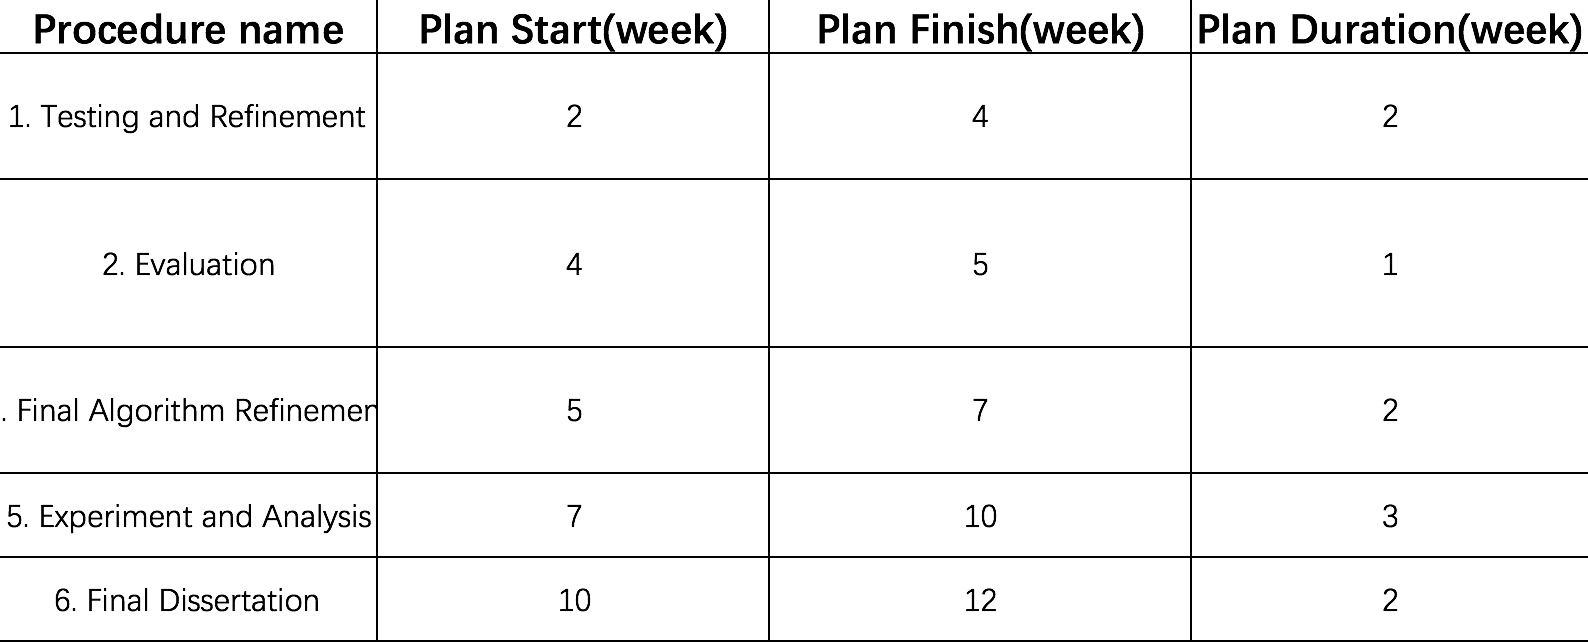
\includegraphics[width=1.0\textwidth]{plan_form.png}
	\caption{plan form\label{fig:plan_form}}
\end{figure}


\begin{figure}[!ht]
	\centering
	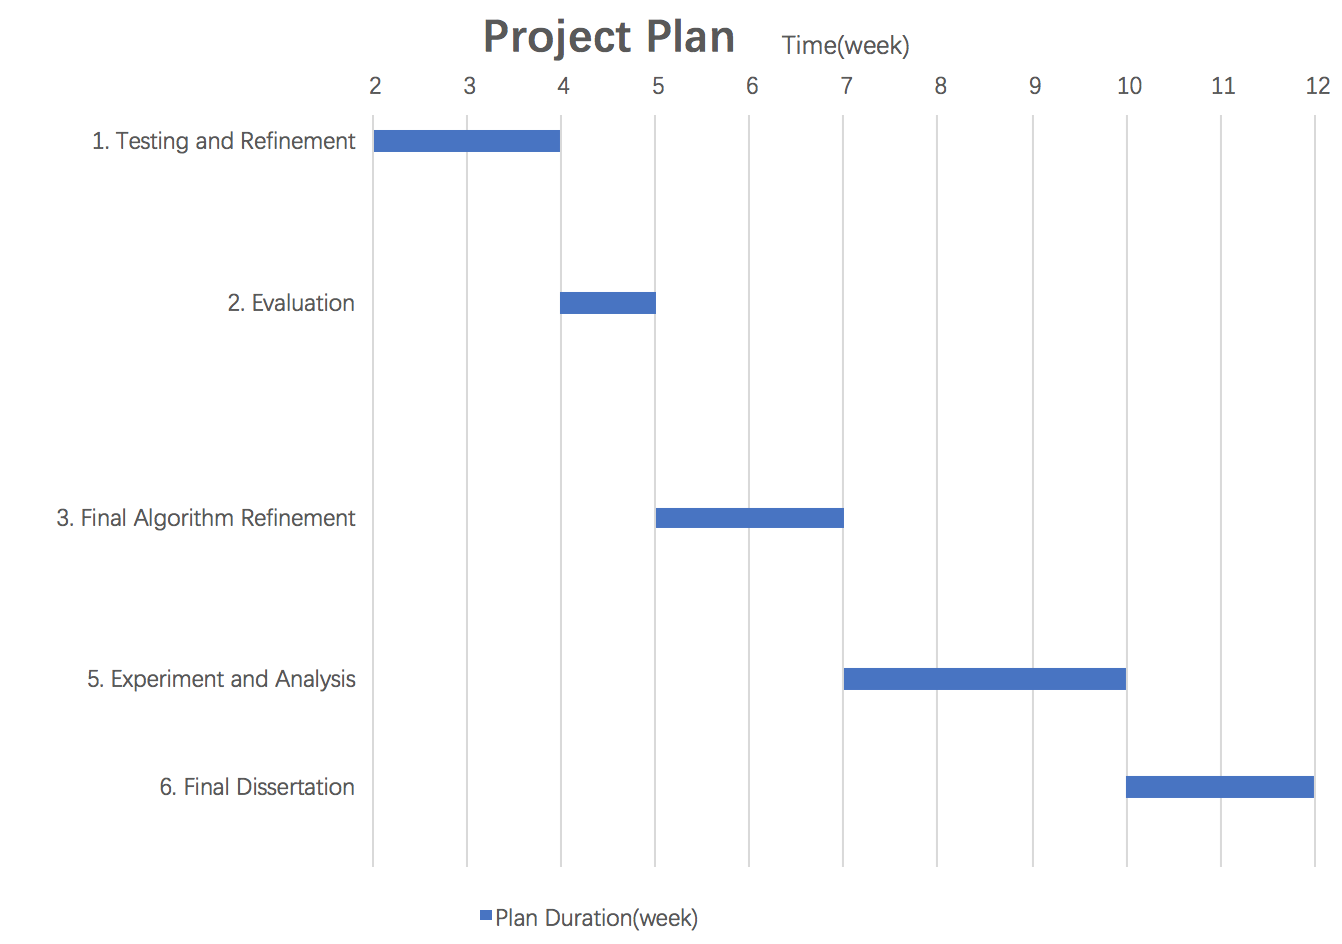
\includegraphics[width=0.8\textwidth]{plan.png}
	\caption{plan for the dissertation\label{plan:lstm}}
\end{figure}



\end{document}
